\ifpdf
    \graphicspath{{figures/}{figures/comparisons}}
\else
    \graphicspath{{figures/}{figures/comparisons}}
\fi

%: ----------------------- name of chapter  -------------------------
\chapter{Problem definition and general implementation aspects}
Summing up when it's hard to determine ideal point correspondences between images, it also is hard to determine the proper solution of essential matrix decomposition. However modern cameras for instance in smartphones have an additional sensors, that allow for tracking position in space. It follows from the analysis of the theory and related works that both epipolar equations and pose estimation techniques can be improved by additional rotation and translation information data.
This is why initially author wanted to resolve issues of \textbf{E} decomposition by direct calculation of \textbf{R} and \textbf{T} from Sensor Fusion data. Seperate tests for rotation and translation accuracy estimations were made and unfortunately, the first attempts to perform reconstruction proved it to be not accurate enough. 
This is where author decided to try few different approaches of combining Sensor Fusion data with already known algorithms. Chapters \ref{chap:recon_sensors} - \ref{chap:enh_5_8_point} document conceptual parts, additional important aspects and tests performed during development of algorithms for cameras rotation and translation estimation created by author's research. 
Chapter \ref{chap:structure_from_motion} includes additional tests performed on images sequence to check their efficiency and influence on 3D spatial (sparse) model creation in pipeline of Structure From Motion methods. But first to help reader go through lecture of this thesis this chapter gives overview of research environment implemented by author.
\section{Requirements}
To perform necessary tests author needed an input in the form of a series of images with additional information about the position of the camera - the euclidean rotation and translation. 
This is why it was necessary to create an mobile application, which would be able to register Sensor Fusion data during images capturing phase.
It wouldn't have to be necessary a smartphone, however in the moment of author's research there was none camera, which would calculate it's rotatation and translation during movement. 
\section{Choosing Environment}
Currently, Android has one of the best and open APIs which allows programmers to acquire sensor fusion data of rotation and linear acceleration. This is also why author's wanted to research particularly, how Android Sensor Fusion can be used to enhance 3D reconstruction techniques.
\\
In order to avoid creating anew all epipolar geometry algorithms, C++ version of OpenCV library was used. However image acquiring process was separated from the model reconstruction. In general, the project was split into two sub-projects: Android for images capturing and df for reconstruction tests. This allowed to save a lot of time in error debugging which is highly difficult in native C++ development on Android. Native code can not be easily breakpointed, which makes it hard to determine, what exactly the error is. Also after every code recompilation, it is necessary to upload application to the device, which usually takes few minutes.
Fortunately once debugged, reconstruction algorithms written in C++ code can be easily ported to Android thanks to Native Development Kit (NDK). 
\section{''Sensor Enhanced Images Camera'' - Android Gradle based project}
In order to capture images and associate them with sensor data, a custom photo capture application called ''Sensor Enhanced Images Camera'' was created.
Using this application, the camera orientation angles can be tracked in real-time. Also linear acceleration, current velocity and relative translation from the location of the last picture taken can be tracked. It was expected that translation calculation error will rise quickly, therefore translation is measured relatively to previously taken image. Also movement heuristic constraint was proposed to avoid unexpected rise of device velocity. In particular this research and applications were adapted for human walking model for translation estimation. This will be explained in detail in Chapter \ref{chap:recon_sensors}.
\subsection{Installation}
In order to compile and distribute Android application, a Gradle based built system was used. This is currently a recommended way to maintain Android-based projects \cite{website:gradle}. 
At present this application supports the devices with Android 4.0 and above only. In order to compile this project it is recommended to install Android Studio, which already contains the required SDK and also has a built-in Gradle support. More information about configuration, compilation and installation steps can be found in README.md in the main catalog of the attached source code. 
\subsection{Project Structure}
Source codes of applications can be found on an attached CD in Folder "Android - Sensor Enhanced Images Camera". In addition, some of the sample datasets were added to the "DataSets" folder in order to allow reader perform evaluations similar to the ones described in the next chapters.
The most two important classes are:
\begin{enumerate}
\item \textbf{CameraSurface.java} - responsible for camera preview setup
\item \textbf{CameraActivity.java} - responsible for User Interface creation, Sensor Fusion data access and capturing pictures with these data. It also includes translation estimation code, which is not a part of Android API and has to be done programatically.
\end{enumerate}
\subsection{User Interface}
As mentioned earlier the program allows to track all necessary external camera parameters like rotation angles and relative position in all axes in real-time. In figure \ref{fig:AndroidScreenShot} it can be seen how the User Interface looks like.
\begin{figure}[h!]
    \centering
    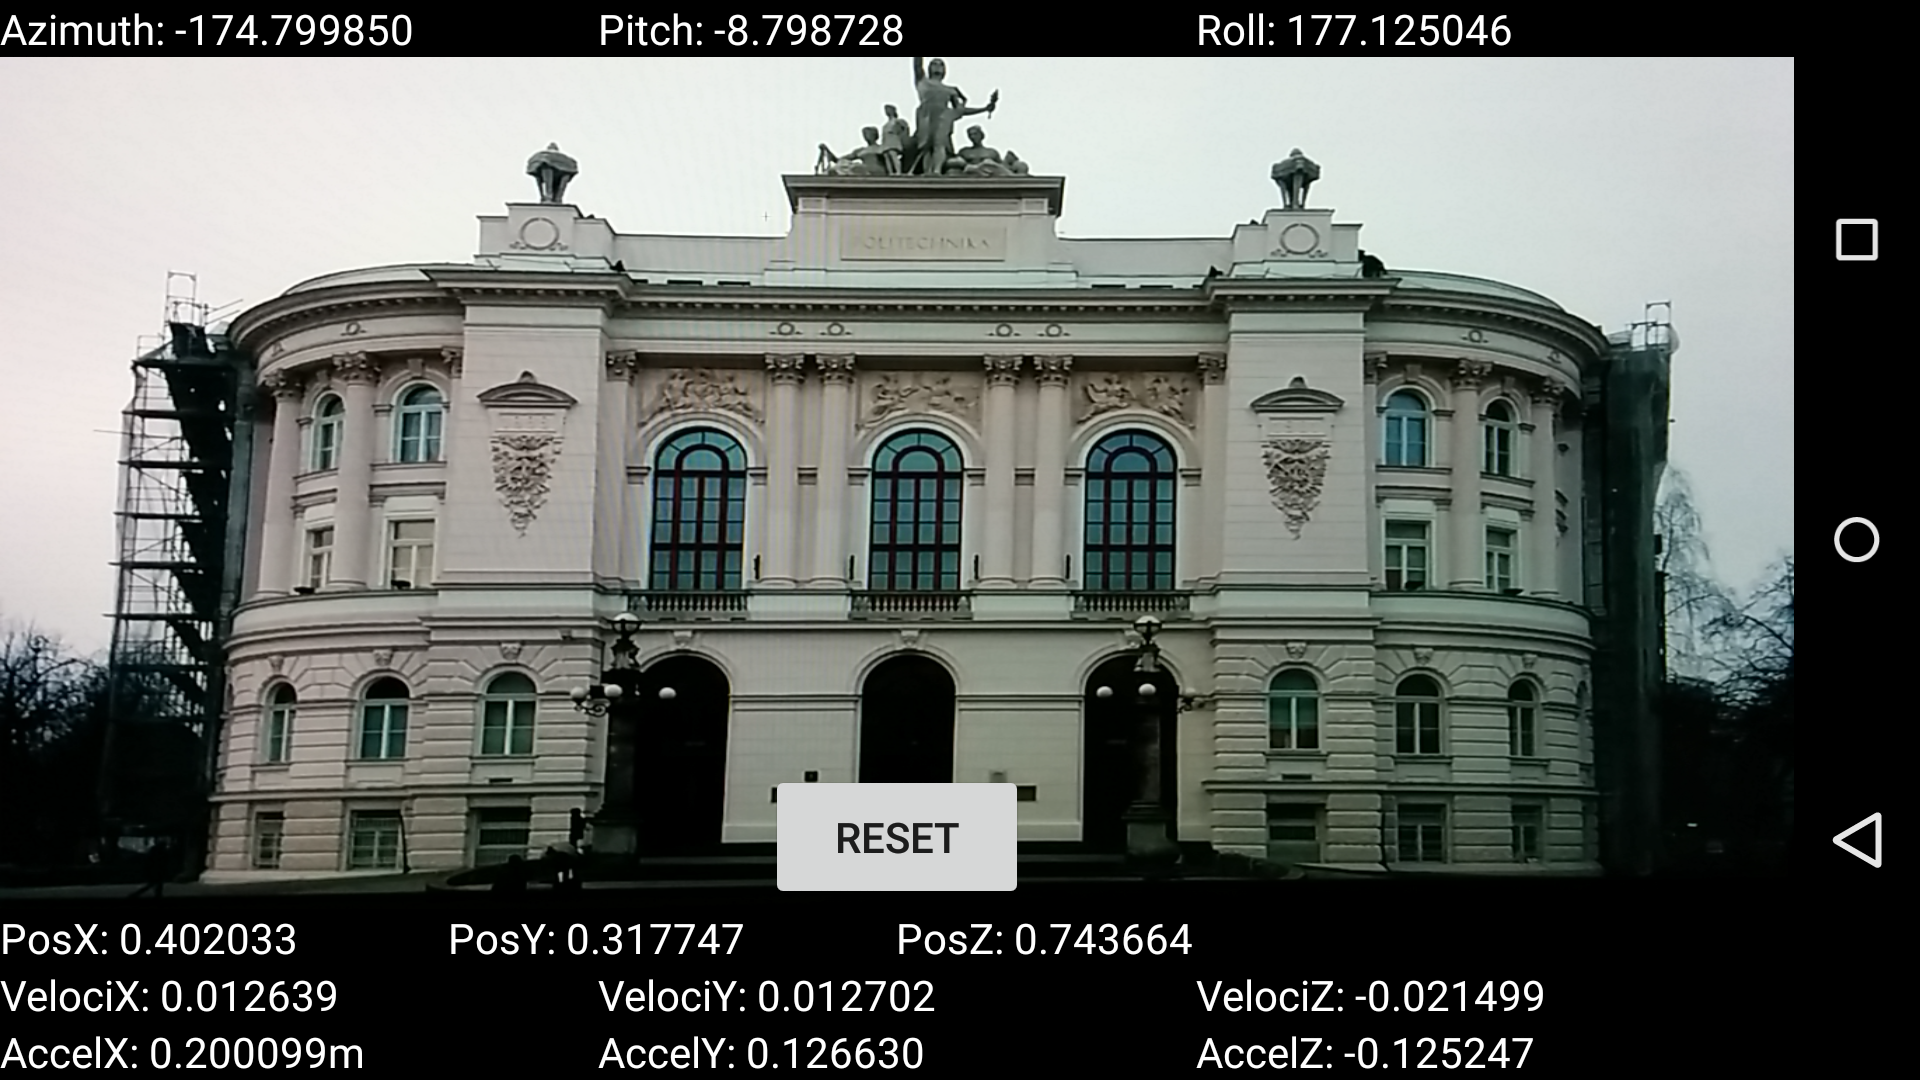
\includegraphics[width=0.8\textwidth]{AndroidScreenShot}
    \caption{Android ''Sensor Enhanced Image Camera'' User Interface overview}
    \label{fig:AndroidScreenShot}
\end{figure}
In order to capture a photo, a user only has to click on the screen center. No additional configuration is required. Reset button can be use to reset translation estimations, when errors are becoming to big. To use the acquired datasets in another program, the smartphone has to be connected to the computer. For each object capture separate folders are created in the main catalog of an internal SD card.
\subsection{Rotation calculation} \label{sec:rot_cal}
Android SDK already has a built-in API which can be used to access sensor fusion data. In particular, for measuring the rotation, $Sensor.TYPE\_ROTATION\_VECTOR$ was used. It returns 9-degree quaternion, which means that it references rotation to geomagnetic north pole. In order to decompose it to Euler angles a helper methods from Android API were in following code fragment used:
\lstset{escapechar=@,style=customjava}
\begin{lstlisting}
import android.hardware.SensorManager;
...
private float[] euclidanAnglesFromQuaternion(float[] quaternion) {
        ...
        //Converts quaternion to 4x4 rotation matrix
        SensorManager.getRotationMatrixFromVector(rotMat, quaternion);
        ...
        //Extracts euclidean Angles in radians (pitch, azimuth, roll)
        SensorManager.getOrientation(rotMat, orientation);
        ...
        return orientation;
}
\end{lstlisting}
\subsection{Custom Sensor Data File format}
Upon the photo capture the current camera rotation and relative translation are saved in a custom JSON file. A corresponding image is saved along with this JSON file in a folder, which is created with actual time suffix upon every program startup. It allows for taking different dataset captures without them being mixed up. \\
As mentioned earlier each photo sensor information is stored in a separate file. By default the following information is stored for each captured image:
\begin{itemize}
\item \textbf{ID}, which indicates order of the photos
\item \textbf{Path}, which relates the path to a corresponding image file
\item \textbf{Euler Angles - pitch, roll, azimuth}
\item \textbf{Relative translation to last taken picture}
\end{itemize} 
All these pieces of information are stored as a list and when the user has completed taking pictures, entire information set is saved into JSON file named sensor.txt. A sample file can be found in the Additional Materials (Listing \ref{lst:json_file}).
\clearpage
\section{''Enhanced 3D Reconstructer'' - OSX CMake-based project}
In order to evaluate algorithms there was a need to prepare a comfortable project environment which would allow for numerical and visual comparison of multiple datasets. CMake was chosen in order to simplify building and compilation process. The entire code architecture was developed and tested on Apple MacbookAir with OSX 10.9 Mavericks. 
\subsection{Installation}
In order to compile this project the following elements need to be installed first:
\begin{itemize}
\item CMake 2.8
\item OpenCV 2.4.10
\item Point Cloud Library (PCL) 1.7 \cite{website:pcl}
\item Boost 1.55
\item cvsba \cite{website:cvsba}
\end{itemize}
\subsection{Project Structure}
Source codes of both applications can be found on an attached CD and in the Github repository at the following web address: \url{https://github.com/KrzysztofWrobel/MasterThesisSource.git}.  In addition, some of the sample datasets were added to the dataset folder in order to allow reader perform evaluations similar to the ones described in the next chapters.
//TODO TODO TODO 

Source codes of applications can be found on an attached CD in Folder ”Android - Sensor Enhanced Images Camera”. In addition, some of the sample datasets were added to the ”DataSets” folder in order to allow reader perform evaluations similar to the ones described in the next chapters. The most two important classes are:
1. CameraSurface.java - responsible for camera preview setup
2. CameraActivity.java - responsible for User Interface creation, Sensor Fusion data access and capturing pictures with these data. It also includes translation estimation code, which is not a part of Android API and has to be done progra-
matically.

\subsection{User Interface}
There are two targets defined in CMake file:
\begin{enumerate}
\item \textbf{Test efficiency}, which was used to evaluate pair reconstruction methods, draw epipolar lines in images and calculate Sampson error distances
\item \textbf{Test reconstruction}, which was used to evaluate proposed initialisation pair reconstruction methods with different pose estimation methods
\end{enumerate}
\subsubsection{Test Efficiency}
There is console interface for reconstruction parameters configuration. To perform necessary tests, where was not need to create graphical interface. The following parameters have to be configured to perform efficiency test, which includes Sampson Errors calculation and epipolar lines visualisations in chosen images:
\begin{enumerate}
\item \textbf{Enhanced Photo Data folder path}
\item \textbf{Initial SIFT features set size}
\end{enumerate}
The calculated execution time and Sampson error measurements are printed to the console output.
\subsubsection{Test reconstruction}
In this case also there is only console interface for reconstruction parameters configuration. All necessary parameters have to be configured from the command-line interface. The following variables need to be configured:
\begin{enumerate}
\item \textbf{Enhanced Photo Data folder path}
\item \textbf{Initial SIFT features set size}
\item \textbf{Init pair reconstruct method}
\begin{itemize}
\item Standard 8-point algorithm
\item Enhanced 8-point algorithm
\item Standard 5-point algorithm
\item Enhanced 5-point algorithm
\item Alternative 3-point translation estimation
\item None (use existing rotations and translations informations)
\end{itemize}
\item \textbf{Pose estimation method:}
\begin{itemize}
\item Standard OpenCV Pose Estimation
\item Rotation enhanced Pose Estimation 
\item Rotation and translation enhanced Pose Estimation
\item None (use existing rotations and translations)
\end{itemize}
\item \textbf{Whether drop outliers or not}
\item \textbf{Whether use Bundle Adjustment or not}
\end{enumerate}
The output received by the user is a reconstructed model in a file with *.asc extension. The reconstructed model is also visible in PCL Visualiser integrated into the code. The user can navigate through the model with mouse and 'F' key, which centres the camera view on a selected point.
\subsection{Rotation matrix generation} \label{sec:rot_gen}
To parse Android generated sensor data file Boost::JsonParser was used. As mentioned earlier, Android saves decomposed Euler angles. In order to properly multiply this angles to acquire a proper rotation matrix the following code inspired by MathWorld Wolfram's definition of Euler angles \cite{website:eulerAngles}. Following listing shows the implementation of equations, that can be found on the pointed website:
\begin{lstlisting}
Mat getRotation3DMatrix(double pitch, double azimuth, double roll) {
    Mat D = (Mat_<T>(3, 3) <<
            cos(roll), -sin(roll), 0,
            sin(roll), cos(roll), 0,
            0, 0, 1);

    Mat C = (Mat_<T>(3, 3) <<
            cos(azimuth), 0, -sin(azimuth),
            0, 1, 0,
            sin(azimuth), 0, cos(azimuth));
    Mat B = (Mat_<T>(3, 3) <<
            1, 0, 0,
            0, cos(pitch), -sin(pitch),
            0, sin(pitch), cos(pitch));
    //Important
    return B * C * D;
}
\end{lstlisting}



% ---------------------------------------------------------------------------
%: ----------------------- end of thesis sub-document ------------------------
% ---------------------------------------------------------------------------

